\chapter{Polynomial Trajectory Optimization}\label{sec:trajectory}


\section{Polynomial Trajectory}\label{sec:polynomial}

Regarding the differentiability of polynomials, they are a profound choice to represent a trajectory. Especially for the use in a differentially flat representation of the UAV dynamics. (Flatness in the proper sense of system theory means that all the states and inputs can be expressed in terms of the flat output and a finite number of its derivative).
Furthermore, the differentiability of polynomials enables the possibility to check the derivatives of the trajectory for bounding violations to avoid input saturation. This saturation-check can be performed during trajectory optimization and therefore guarantees the feasibility of the resulting trajectory.

\section{Optimization}\label{sec:optimization}

The goal of this master thesis is to optimize a trajectory which passes through waypoints (also called vertices or nodes) which are defined in advance. This waypoints can be chosen manually or by a path-finding algorithm such as RRT* which will be discussed in chapter \ref{chap:RRT}.
Furthermore, not only the waypoints (i.e. the position) can be fixed in advance but also its derivatives (such as speed, acceleration etc.). The position and its derivatives are then utilized as the equality constrains for a QP (explained in Section \ref{sec:quadratic}).

\subsection{Cost Function}\label{sec:cost}

Optimization for the purpose of trajectory planning means to minimize a cost function. The cost function in this case is a combination of temporal and geometric cost. The geometric cost penalizes the square of the derivatives of the trajectory. In this master thesis the geometric cost is represented by the squared snap which guarantees a trajectory without abrupt  control inputs. \newline
The temporal cost is simply the total trajectory time multiplied by a user chosen factor $k_T$ which determines the aggressiveness of the resulting trajectory. The impact of  $k_T$  can be seen in equation \ref{equ:total_cost} which represents the combined geometric and temporal cost. \newline

To express the geometric cost in a compact way one can utilize the Hessian matrix $Q$. The Hessian matrix is defined as a squared matrix of second-order partial derivatives which follows from differentiation a function with respect to each of its coefficients, in this instance the polynomial coefficients. The geometric cost function $J(T)$ for one segment with the duration $T$ can now be written as

\begin{equation}
J(T)  = p^T \cdot Q(T) \cdot p
\end{equation}

where $Q(T)$ is the Hessian matrix for a fixed segment time $T$. $p$ is the vector containing the coefficients of the polynomial trajectory. \newline

If the trajectory consists of more than one segment the Hessian matrix has to be extended to a block-diagonal matrix. The geometric cost function for multiple segments with fixed but individual segment times $T_i$ can be written as

\begin{equation}
J(T) =
\begin{bmatrix}
   p_1 \\
\vdots \\
  p_n
\end{bmatrix}^T
\cdot
\begin{bmatrix}
   Q_1(T_1) &  &  \\
    & \ddots &  \\
   & & Q_n(T_n)
\end{bmatrix} 
\cdot
\begin{bmatrix}
   p_1 \\
\vdots \\
  p_n
\end{bmatrix}
\label{equ:cost}
\end{equation}


\subsection{Polynomial Optimization as a Constrained QP}

The cost function in equation \ref{equ:cost} has to be minimized under constrains since we want to fix things like start or end position. In a first intuitive approach the constraints on the endpoint derivatives are utilized in a constrained QP. Therefore, a mapping matrix $E$ between endpoint derivatives and polynomial coefficients is needed. The resulting equality constraint for the $i^{th}$ segment can be written as

\begin{equation}
E_i \cdot p_i = d_i
\label{equ:mapping}
\end{equation}

where $p$ is the vector containing the polynomial coefficients and $d$ is the vector containing the endpoint derivatives. Regarding the total number of segments of the trajectory, equation \ref{equ:mapping} can be written in matrix form:

\begin{equation}
\begin{bmatrix}
   E_1 &  &  \\
    & \ddots &  \\
   & & E_n
\end{bmatrix} 
\cdot
\begin{bmatrix}
   p_1 \\
\vdots \\
  p_n
\end{bmatrix}
=
\begin{bmatrix}
   d_1 \\
\vdots \\
  d_n
\end{bmatrix}
\end{equation} 

The constrained QP is suitable for a small amount of segments but gets ill-conditioned for a large amount of segments and therefore large matrices. Especially if there are matrices which are close to singularity and have coefficients which are close to zero, the constrained QP can get numerical unstable.

\subsection{Polynomial Optimization as a Unconstrained QP}\label{sec:polynomialQP}

To avoid the numerical instability of a constrained QP the optimization problem is converted into a unconstrained QP. To achieve this, the polynomial coefficients $p_i$ from equation \ref{equ:cost} have to be substituted by the endpoint derivatives $d_i$ which are now the new optimization variables. The cost function of the unconstrained QP can now be written as 

\begin{equation}
J =
\begin{bmatrix}
   d_1 \\
\vdots \\
  d_n
\end{bmatrix}^T
\cdot
\begin{bmatrix}
   E_1 &  &  \\
    & \ddots &  \\
   & & E_n
\end{bmatrix} ^{-T}
\cdot
\begin{bmatrix}
   Q_1 &  &  \\
    & \ddots &  \\
   & & Q_n
\end{bmatrix} 
\cdot
\begin{bmatrix}
   E_1 &  &  \\
    & \ddots &  \\
   & & E_n
\end{bmatrix} ^{-1}
\cdot
\begin{bmatrix}
   d_1 \\
\vdots \\
  d_n
\end{bmatrix}
\label{equ:uncon_cost}
\end{equation}

where $Q_i$ is the Hessian matrix according to the $i^{th}$ segment time $T_i$.\newline

As mentioned above, the endpoint derivatives are the new optimization variables. Due to the equality constrains some of the endpoint derivatives are already specified consequently reducing the number of optimizations variables. Expediently, the endpoint derivatives are divided in fixed derivatives $d_f$ and unspecified derivatives $d_p$ and then reordered using the matrix $C$ which consists of zeros and ones. After reordering the endpoint derivatives equation \ref{equ:uncon_cost} can be rewritten as

\begin{equation}
J =
\begin{bmatrix}
   d_f \\
  d_p
\end{bmatrix}^T
\underbrace{C^T E^{-T} Q E^{-1} C}_\text{R}
\begin{bmatrix}
   d_f \\
  d_p
\end{bmatrix}
\label{equ:R_cost}
\end{equation}

where the product of the reordering matrix $C$, the mapping matrix $E$ and the Hessian matrix $Q$ can be expressed as a single Matrix $R$. The matrix $R$ for his part can be divided into four submatrices according to the fixed and unspecified endpoint derivatives which modifies equation \ref{equ:R_cost} as follows:

\begin{equation}
J =
\begin{bmatrix}
   d_f \\
  d_p
\end{bmatrix}^T
\begin{bmatrix}
   R_{ff} & R_{fp} \\
  R_{pf} & R_{pp}
\end{bmatrix}
\begin{bmatrix}
   d_f \\
  d_p
\end{bmatrix}
\label{equ:Rxx_cost}
\end{equation}

Partially differenting equation \ref{equ:Rxx_cost} with respect to the unspecified derivatives $d_p$ and equate it to zero yields the optimized/minimized unspecified derivatives $d_p^*$ 

\begin{equation}
d_p^* = - R_{pp}^{-1} \cdot R_{fp}^T \cdot d_f
\label{equ:dpstar}
\end{equation}

as a function of the fixed derivatives $d_f$ and two of the submatrixes ($R_{pp}, R_{fp}$) of $R$.


\subsection{Initial Solution}\label{sec:initialSolution}

Equation \ref{equ:dpstar} can now be used to compute the initial solution. As can be seen in equation \ref{equ:uncon_cost}, the Hessian matrix for the  $ i^{th}$ segment $Q_i$ depends on the segment time $T_i$. Thus, all the segment times have to be defined in advance. For the initial solution the segment times are calculated based on the Euclidean distance $d_{norm}$ and on the user specified maximal speed ($v_{max}$) and maximal acceleration ($a_{max}$). \newline

Basically the segment time is determined by the term $d_{norm}/v_{max} \cdot 2$ which is twice the time the UAV would need for a segment by flying the whole distance at maximal speed. Although this is a good estimation for long segments, for shorter ones the time needed to accelerate gets significant. In order to incorporate acceleration time, a multiplier which is zero for long segments and unequal to zero for short ones is added. The segment time $T_i$ for the $i^{th}$ segment can be computed according to 

\begin{equation}
T_i = \frac{d_{norm_i}}{v_{max}} \cdot 2 \cdot \left( 1 + 6.5 \cdot \frac {v_{max}}{a_{max}} \cdot \frac{1}{e^{\frac{d_{norm_i}}{v_{max}} \cdot 2}} \right)
\label{equ:segmentTime}
\end{equation}

where $d_{norm_i}$ is the Euclidean distance of the $i^{th}$ segment, $v_{max}$ the user specified maximal velocity and $a_{max}$ the user specified maximal acceleration. The fraction $v_{max}/a_{max}$ gives an idea how much time is needed to accelerate to maximum velocity whereas $6.5$ is a empirical weighting factor. \newline

The result from equation \ref{equ:segmentTime} is depicted in figure \ref{pic:timeEstimation} whereat the $x$-axis represents the Euclidean distance $d_{norm}$ and the $y$-axis represents the segment time $T$. For this plot the user specified limitation on speed has been set to $v_{max} = 3 \frac{m}{s}$  and the limitation on acceleration has been set to  $a_{max} = 5 \frac{m}{s^2}$. The dashed green line represents the term $d_{norm}/v_{max} \cdot 2$ and serves as a reference. The blue graph is the exact representation of equation \ref{equ:segmentTime}. 

\begin{figure}[H]
   \centering
   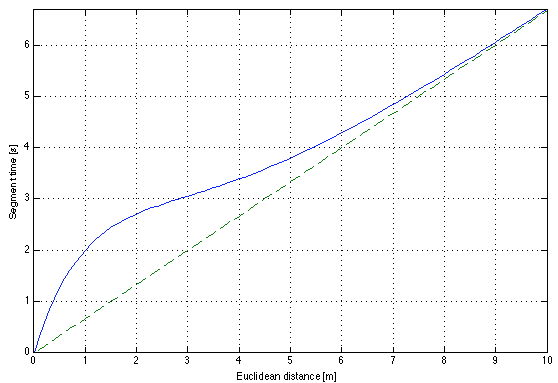
\includegraphics[width=1\textwidth]{pics/time_estimation.png}
   \caption{The segment time $T$ depends on the Euclidean distance $d_{norm}$ of a segment as well as on the max. velocity $v_{max}$ and the max. acceleration $a_{max}$. For short segments the acceleration time is incorporated.}
   \label{pic:timeEstimation}
\end{figure}

Once the segment times are calculated, the initial snap minimized solution can be computed according to equation \ref{equ:dpstar}. The initial solution for a 3 dimensional problem with 4 segments is depict in figure \ref{pic:initialSolution}. The start and goal of the trajectory is the origin of the Cartesian coordinate system (0/0/0). For both, start and goal state, the velocity, the acceleration, the jerk and the snap are fixed and set to zero. For all the other sampling points (vertices) the derivatives are unspecified. The Cartesian coordinates of the sampling points are chosen manually and are listed in the following table: 


\begin{center}
    \begin{tabular}{ | l | c | c | c |}
    \hline
    Waypoint & x-coordinate & y-coordinate & z-coordinate\\ \hline
    Start-Vertex & 0 & 0 & 0 \\ \hline
    Vertex 1 & 5 & 1 & -4\\ \hline
   Vertex 2 & 3 & -2 & 1\\ \hline
   Vertex 3 & -1 & 2 & 3\\ \hline
    Goal-Vertex & 0 & 0 & 0\\
    \hline
    \end{tabular}
    \label{tab:vertices}
\end{center}







Figure \ref{pic:initialSolution} a) shows the position (i.e. the Cartesian coordinates) whereby each of the 3 dimensions is depicted as a single graph. The Cartesian coordinates from the above-noted table are depicted as circles. Plot b) shows the velocity of the individual direction as a solid graph. Additional, the velocity in the three-dimensional space (i.e. the Euclidean norm of the velocity vector) is depicted as a dashed graph. \linebreak 
Plot c) is constructed similarly but depicts the acceleration in the individual directions (solid) and the acceleration in the three-dimensional space (dashed). Furthermore the limitation ($v_{max} = 3 \frac{m}{s}$ and $a_{max} = 2 \frac{m}{s^2}$ for this problem) are depicted.





%The $x$-axis for all the 3 plots is the time. The 3 graphs in the first subplot represent the 3 dimension where the colors are different for each segment. In the second and third subplot, there are also 3 graphs representing a dimension but also a fourth, thicker graph which represents the 2-norm of the velocity respectively the acceleration. Furthermore the limitation ($v_{max} = 3 \frac{m}{s}$ and $a_{max} = 2 \frac{m}{s^2}$ for this problem) are depicted.

\begin{figure}[H]
   \centering
   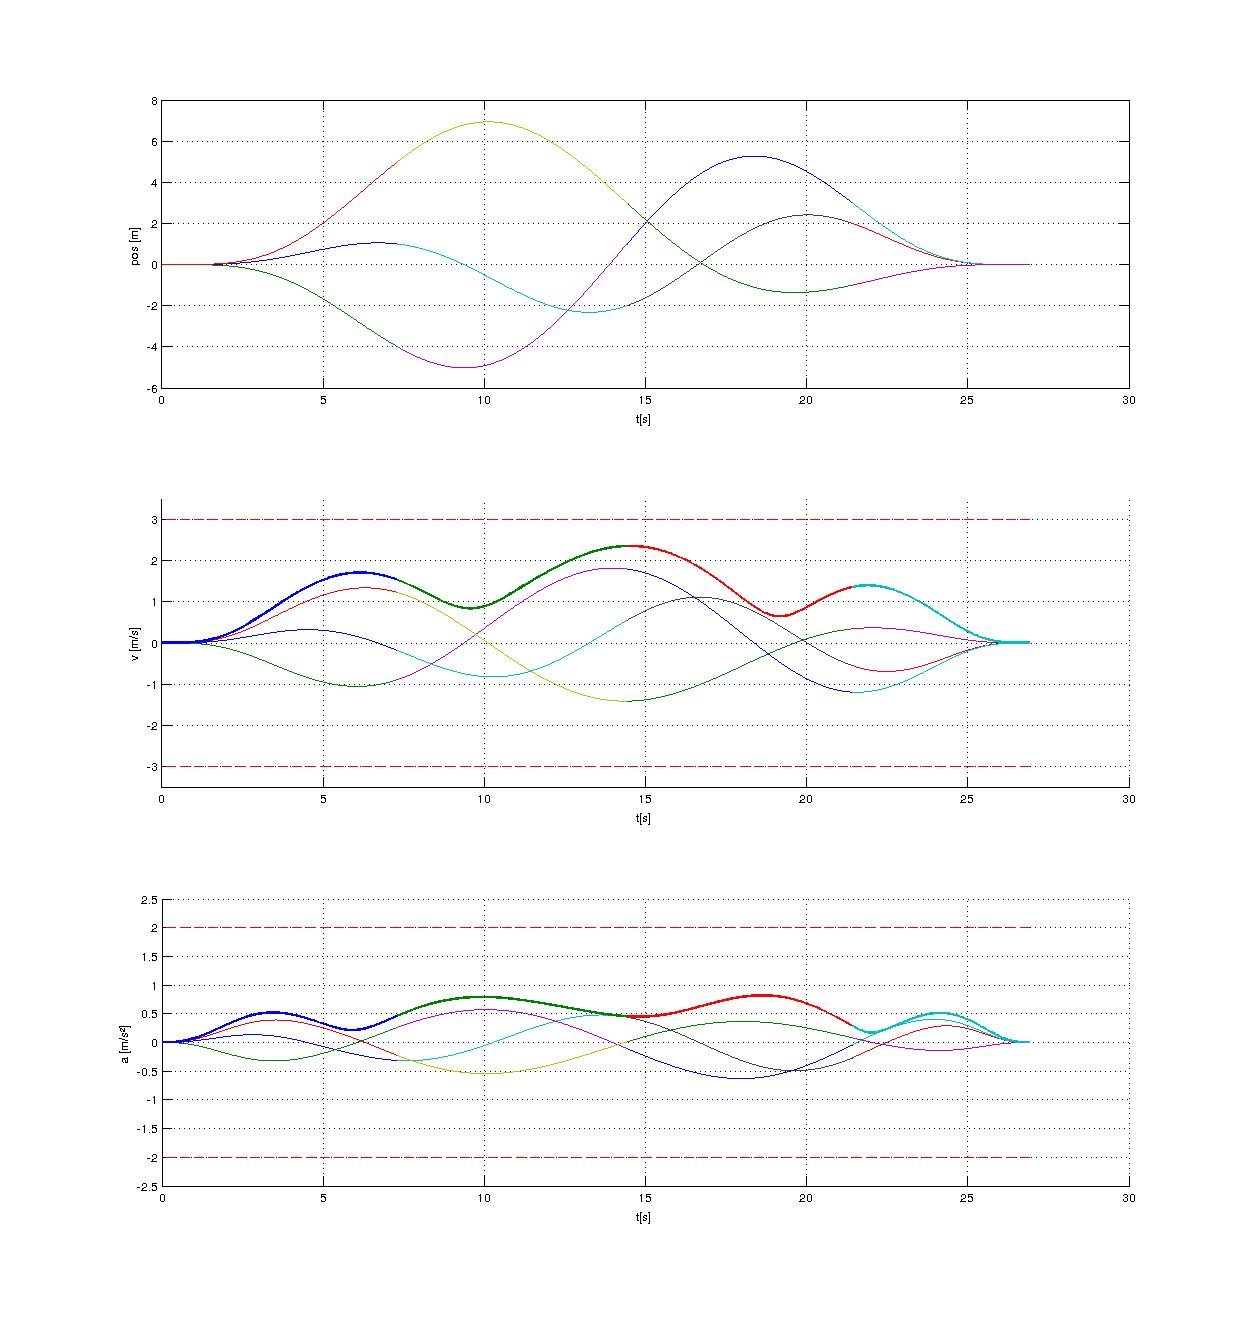
\includegraphics[width=1\textwidth]{pics/initial.jpg}
   \caption{Initial solution of a trajectory with 4 segments: Plot a) shows the position (i.e. the Cartesian coordinates). Plot b) shows the velocity and plot c) the acceleration. A dashed graph represents the velocity respectively the acceleration in the three-dimensional space.}
   \label{pic:initialSolution}
\end{figure}

The total time of the initial trajectory is the sum of the individual segment times and therefore defined by equation \ref{equ:segmentTime}. Since equation \ref{equ:segmentTime} does not incorporate the circumstances from one segment to an other it is likely to find a better trajectory (i.e. a trajectory with a smaller total cost) with the same total time but a different ratio between the segment time. Moreover there is no possibility to adjust the aggressiveness of the initial solution since the segment times are calculated up front. 
Recapitulating, the modification of the individual segment times and therefore the modification of the ratio of the segment times can lead to a better solution. Supplementary, the modification of the individual segment times gives us the opportunity to adjust the aggressiveness of a trajectory.



\subsection{Time Allocation}\label{sec:penalty}

So fare, only the geometric cost (i. e. the squared snap) was included in the cost function defined in equation \ref{equ:Rxx_cost}. Minimization of the geometric cost ensures a smooth trajectory without abrupt input signal but has no effect on the aggressiveness of a trajectory. Therefore equation \ref{equ:Rxx_cost} has to be extended by the temporal cost (i.e. the sum of the segment times) which results in the total cost $J_{total}$

\begin{equation}
J_{total} =
\begin{bmatrix}
   d_f \\
  d_p
\end{bmatrix}^T
\begin{bmatrix}
   R_{ff} & R_{fp} \\
  R_{pf} & R_{pp}
\end{bmatrix}
\begin{bmatrix}
   d_f \\
  d_p
\end{bmatrix}
+ k_T \cdot \sum_{i=1}^N T_i
\label{equ:total_cost}
\end{equation}

where $k_T$ is a user specified penalty on time and $T_i$ is the segment time of the $i^{th}$ segment. \newline

Since a hight value for $k_T$ leads to a trajectory with a brief total trajectory time and a small value for $k_T$ leads to a trajectory with a long total trajectory time, the user specified penalty on time $k_T$ enables the adjustment of the aggressiveness of a trajectory. \newline



The geometric cost function in equation \ref{equ:Rxx_cost} has only the unspecified endpoint derivatives $d_p$ as optimization variables. This optimization problem can be solved analytically as performed in equation \ref{equ:dpstar}. The cost function in equation \ref{equ:total_cost} has the segment times $T_i$ as additional optimization variables. Meaning the segment times $T_i$ are directly represented in the cost function and not only indirectly via the Hessian matrices $Q_{T_i}$. Since the segment times are now optimization variables, the Hessian matrices $Q_{T_i}$ are no longer defined in advance and the problem cannot be solved analytically. Due to that a nonlinear solver is used. In this master thesis NLopt,  a open-source library for nonlinear optimization, is applied. The unspecified endpoint derivatives $d_p$ and the segment times $T_i$ of the initial solution are the initial values for the nonlinear solver. Hence, the computational cost of the nonlinear optimization is highly depending on the quality of the initial solution. \newline

The termination condition of the optimization can be specified by the optimization variables as well as by the total cost. Generally, the termination conditions are formulated relative to the current value(s). For instance, if the relative termination condition for the total cost $J_{rel}$ is set to $0.01$ the optimization ends if the total cost changes less than a percent during an iteration. The relative termination condition for the optimization variables $x_{rel}$ is only fulfilled if all of the optimization variables change less then the threshold. Additionally, an absolute termination condition $x_{abs}$ is applied to the optimization variables but is only called into action if one or several optimization variables are close to zero and the relative criteria therefore don't work properly. Two additional options are the limitation of the number of optimization iterations and the limitation of the duration of the optimization.
During the optimization the constraints on velocity and acceleration are checked every iteration. \newline






The result of the nonlinear optimization is depicted in figure \ref{pic:optimizedSolution}. As can be seen in plot a) the trajectory passes the same waypoints as in Figure \ref{pic:initialSolution}, i.e. the waypoints which are listed in the table in section  \ref{tab:vertices}. The optimized trajectory only needs 18 seconds where as the initial solution required 27 second from start to goal. Figure \ref{pic:optimizedSolution} b) shows the velocity of the individual direction as a solid graph. Additional, the velocity in the three-dimensional space (i.e. the Euclidean norm of the velocity vector) is depicted as a dashed graph. The dashed graph tangents the maximal velocity ($v_{max} = 3 m/s$ in this example) partially. The shorter trajectory time and the exploitation of the limits illustrates that the optimized trajectory is more aggressive then the initial trajectory, \newpage

The same effect of exploiting the limits can be seen in plot c). Similar to plot b), plot c) shows the acceleration of the individual direction as a solid graph and the acceleration in the three-dimensional space as a dashed graph.





\begin{figure}[h]
   \centering
   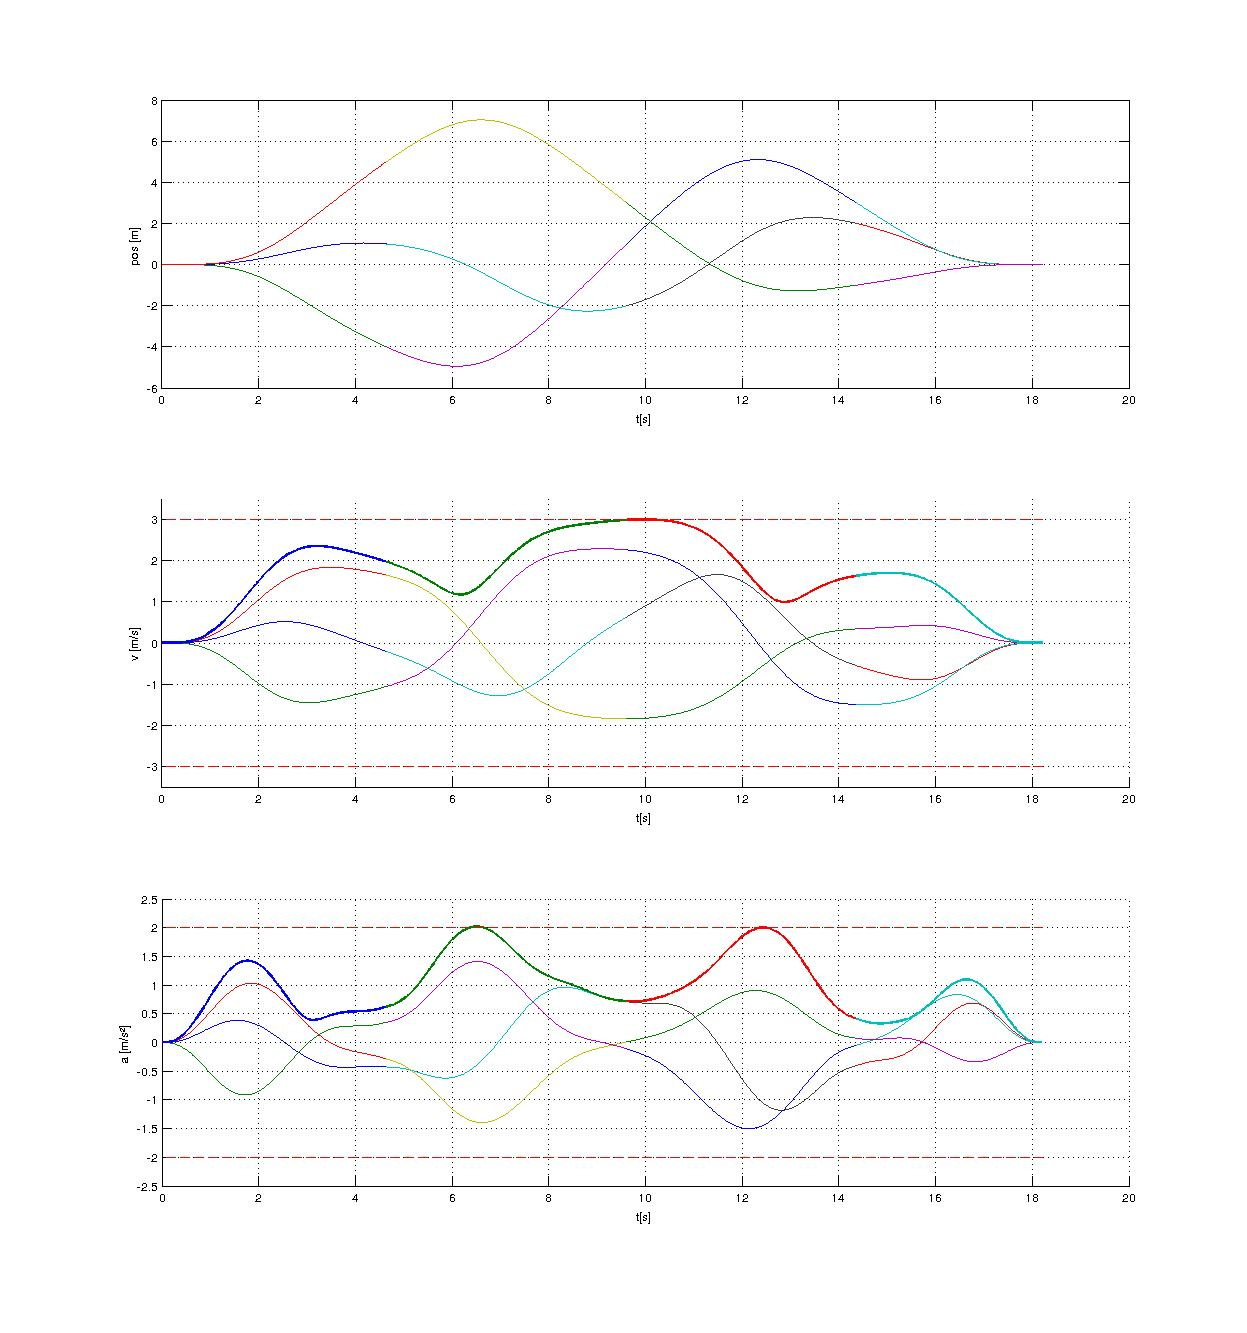
\includegraphics[width=1\textwidth]{pics/optimized.jpg}
   \caption{Optimized solution of a trajectory with 4 segments: Plot a) shows the position (i.e. the Cartesian coordinates). Plot b) shows the velocity and plot c) the acceleration. A dashed graph represents the velocity respectively the acceleration in the three-dimensional space.}
   \label{pic:optimizedSolution}
\end{figure}

\section{Reduce the Optimization Variables}

TODO



%\begin{figure}[h]
%   \centering
%   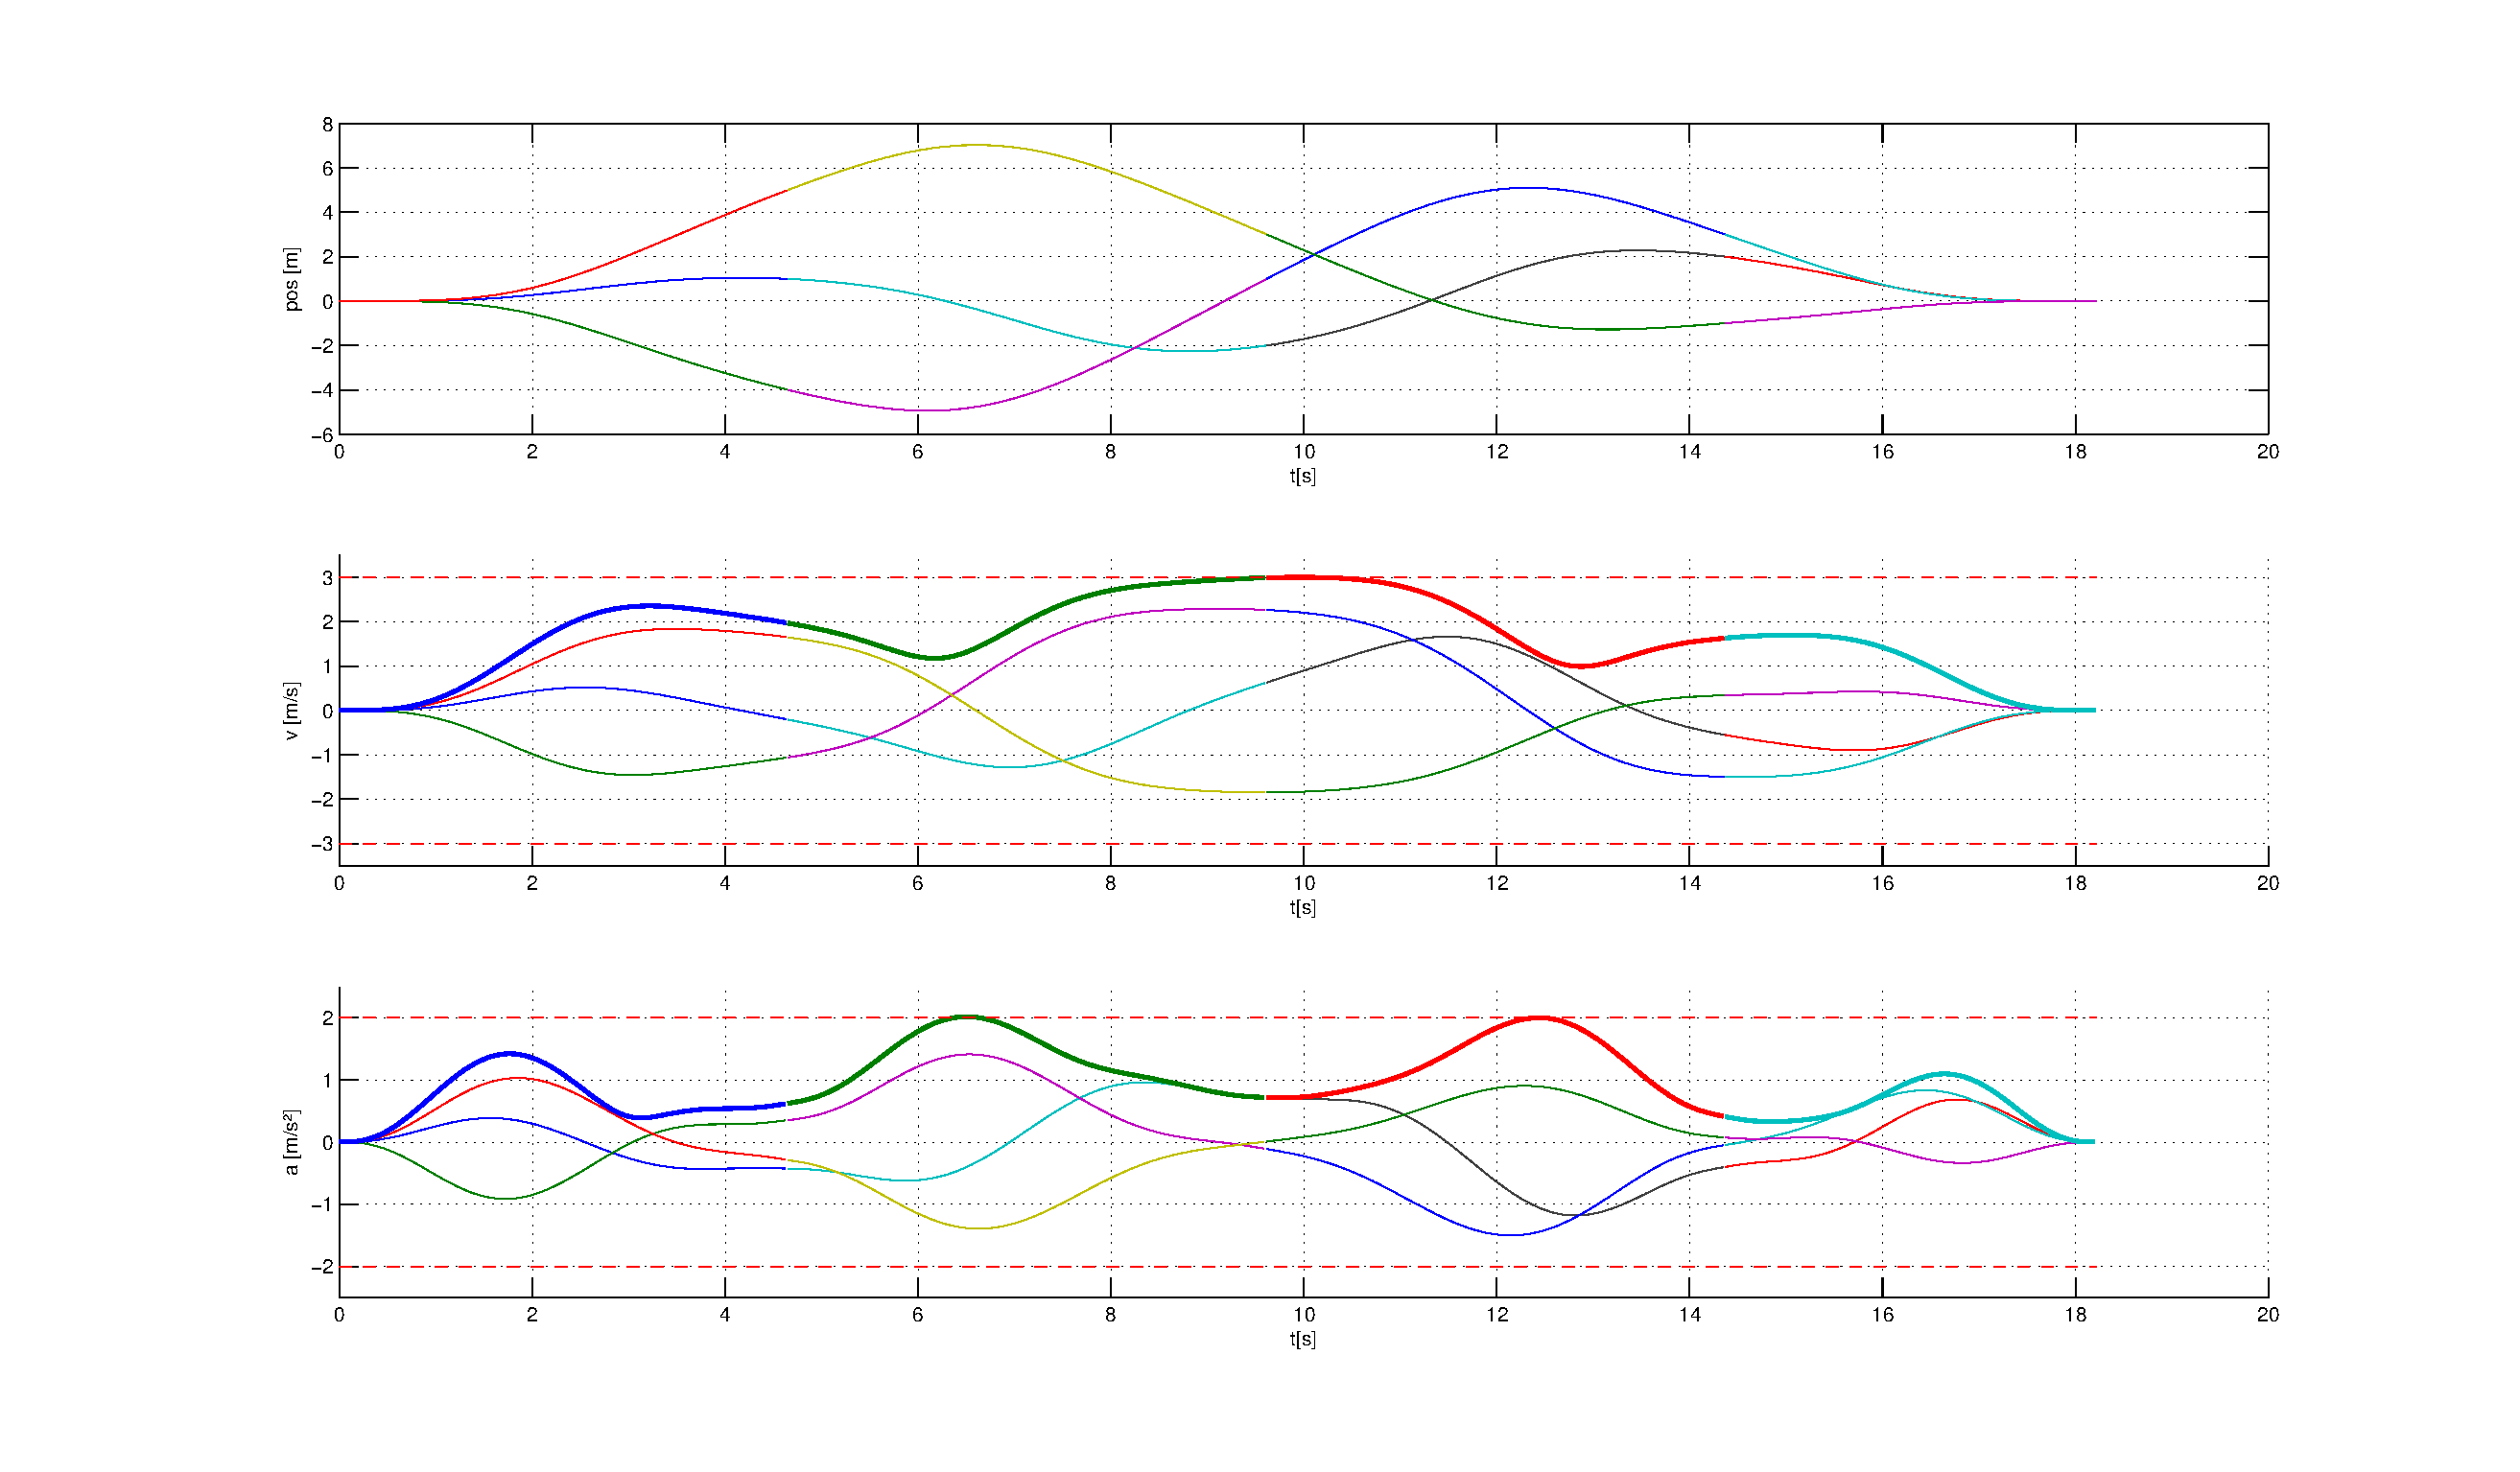
\includegraphics[width=1\textwidth]{pics/optimized.eps}
%   \caption{Ein Bild.}
%\end{figure}
%
%
%\begin{figure}[h]
%   \centering
%   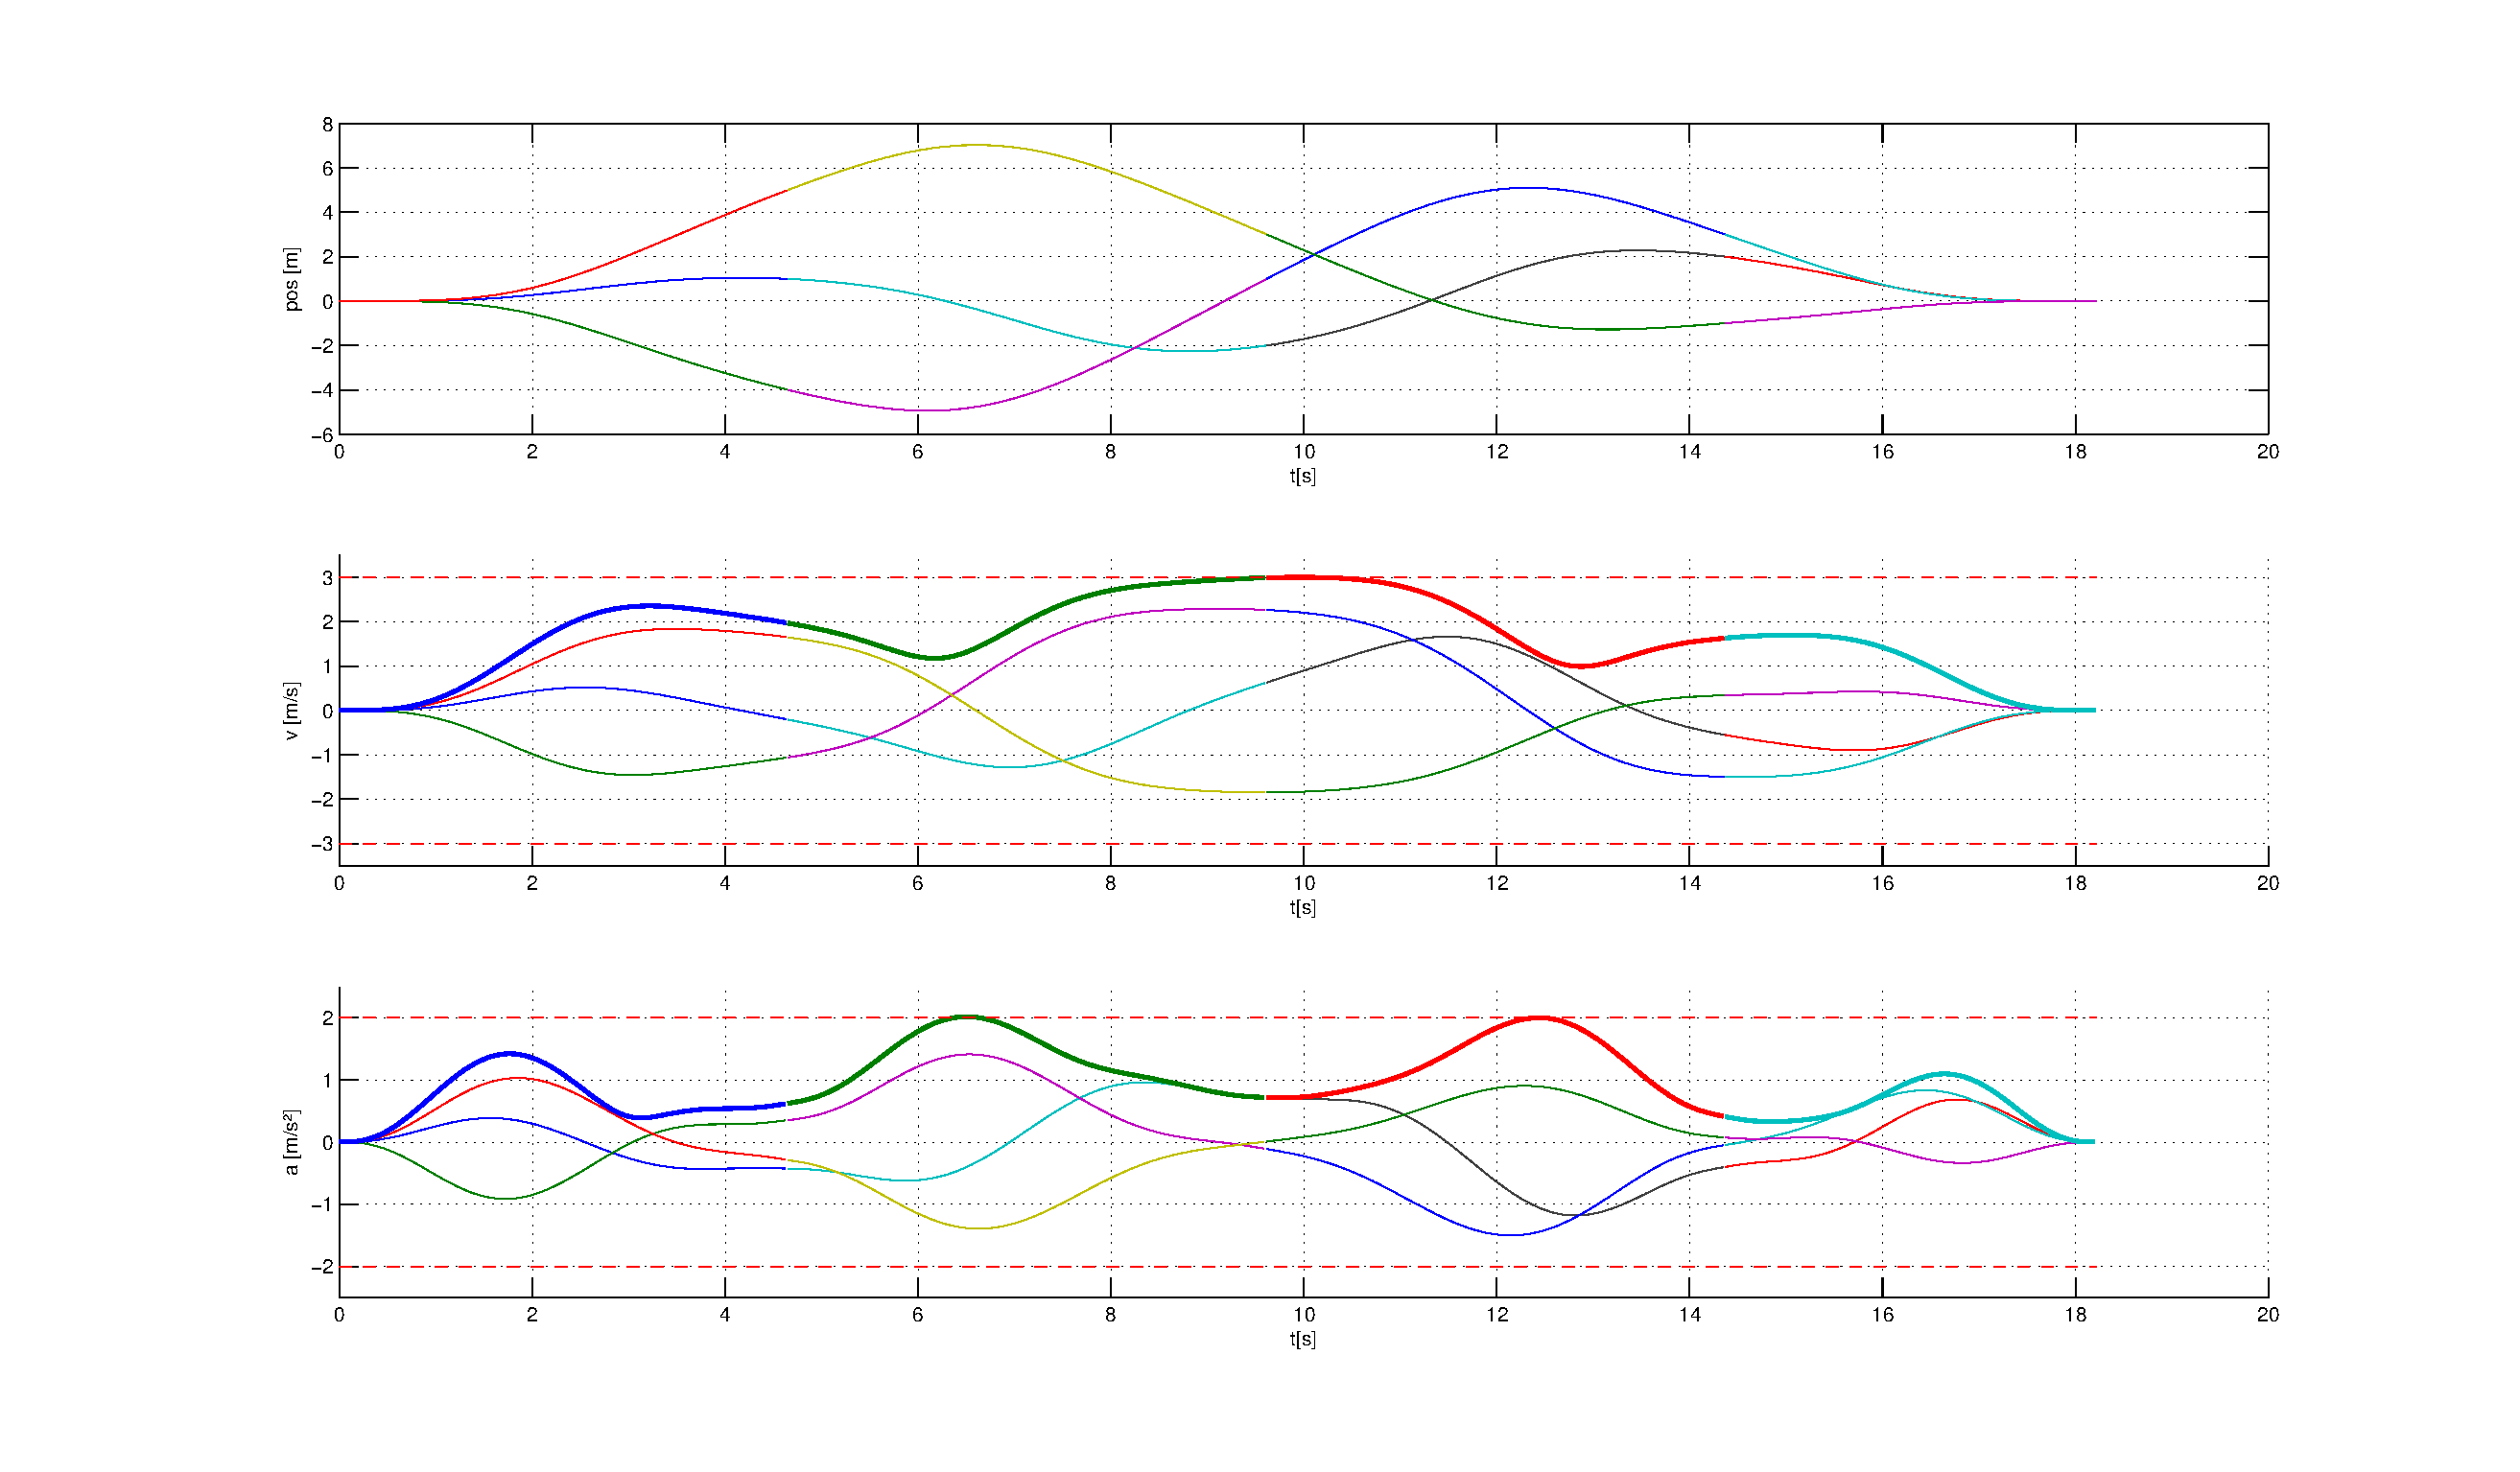
\includegraphics[scale=0.3]{pics/optimized.eps}
%   \caption{Ein Bild.}
%\end{figure}



%\begin{figure}[h]
%   \centering
%   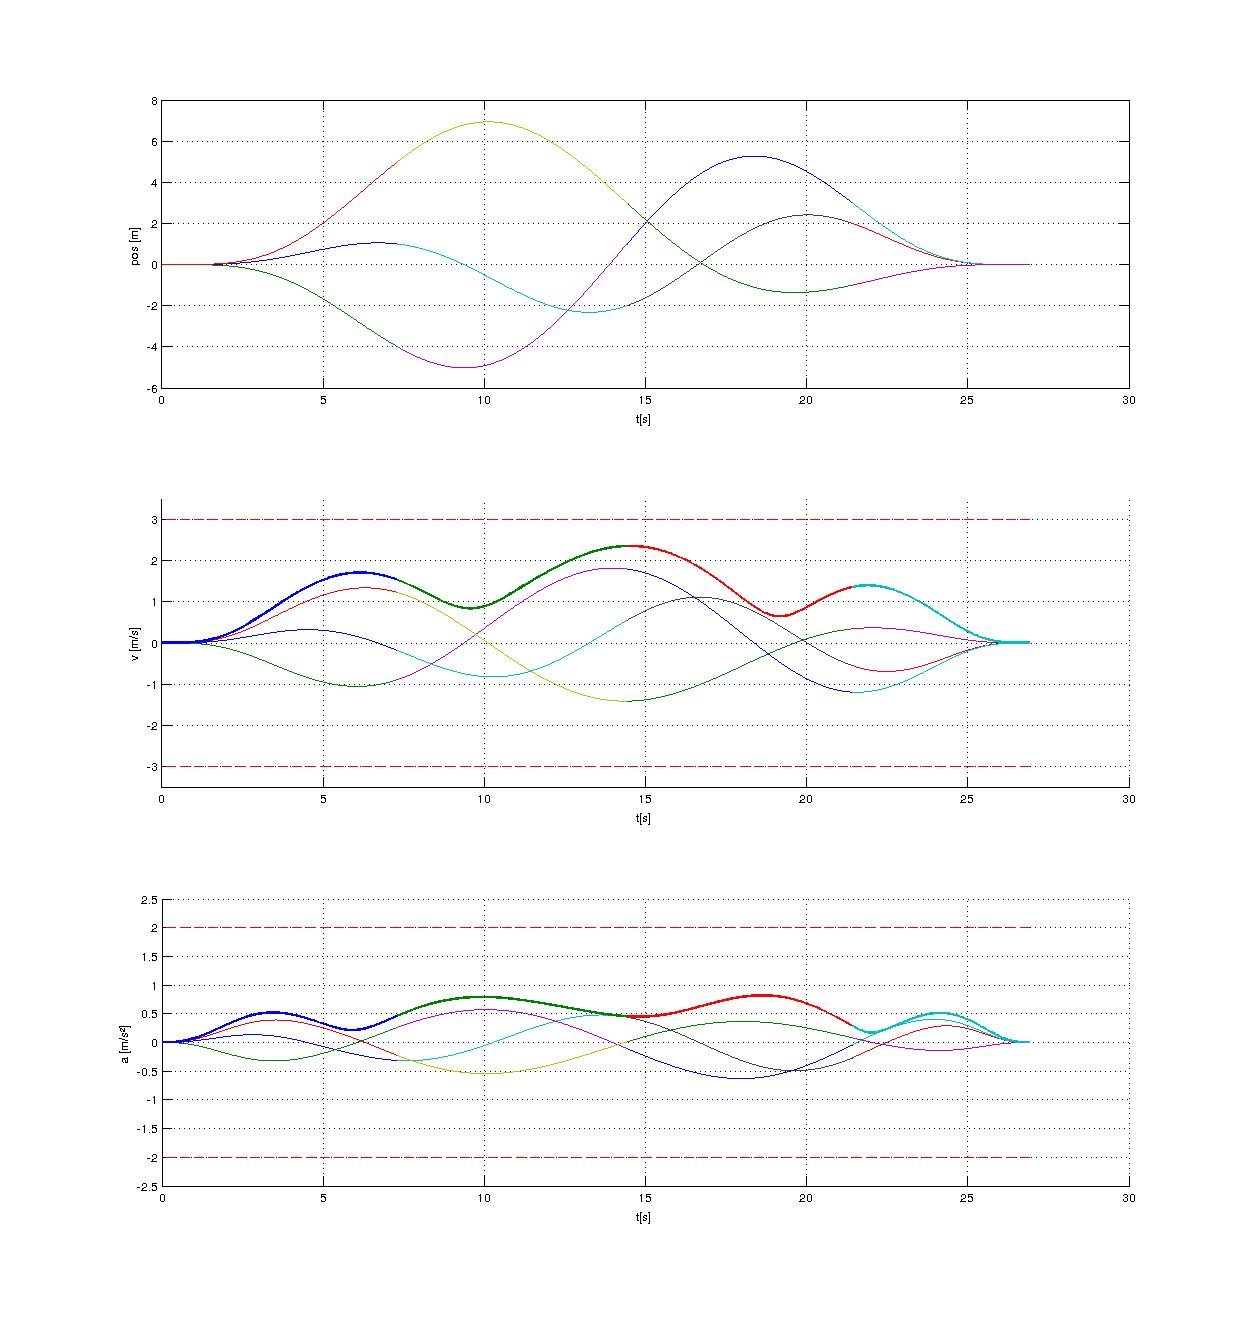
\includegraphics[width=1\textwidth]{pics/initial.eps}
%   \caption{Ein Bild.}
%\end{figure}

%\begin{figure}[h]
%   \centering
%   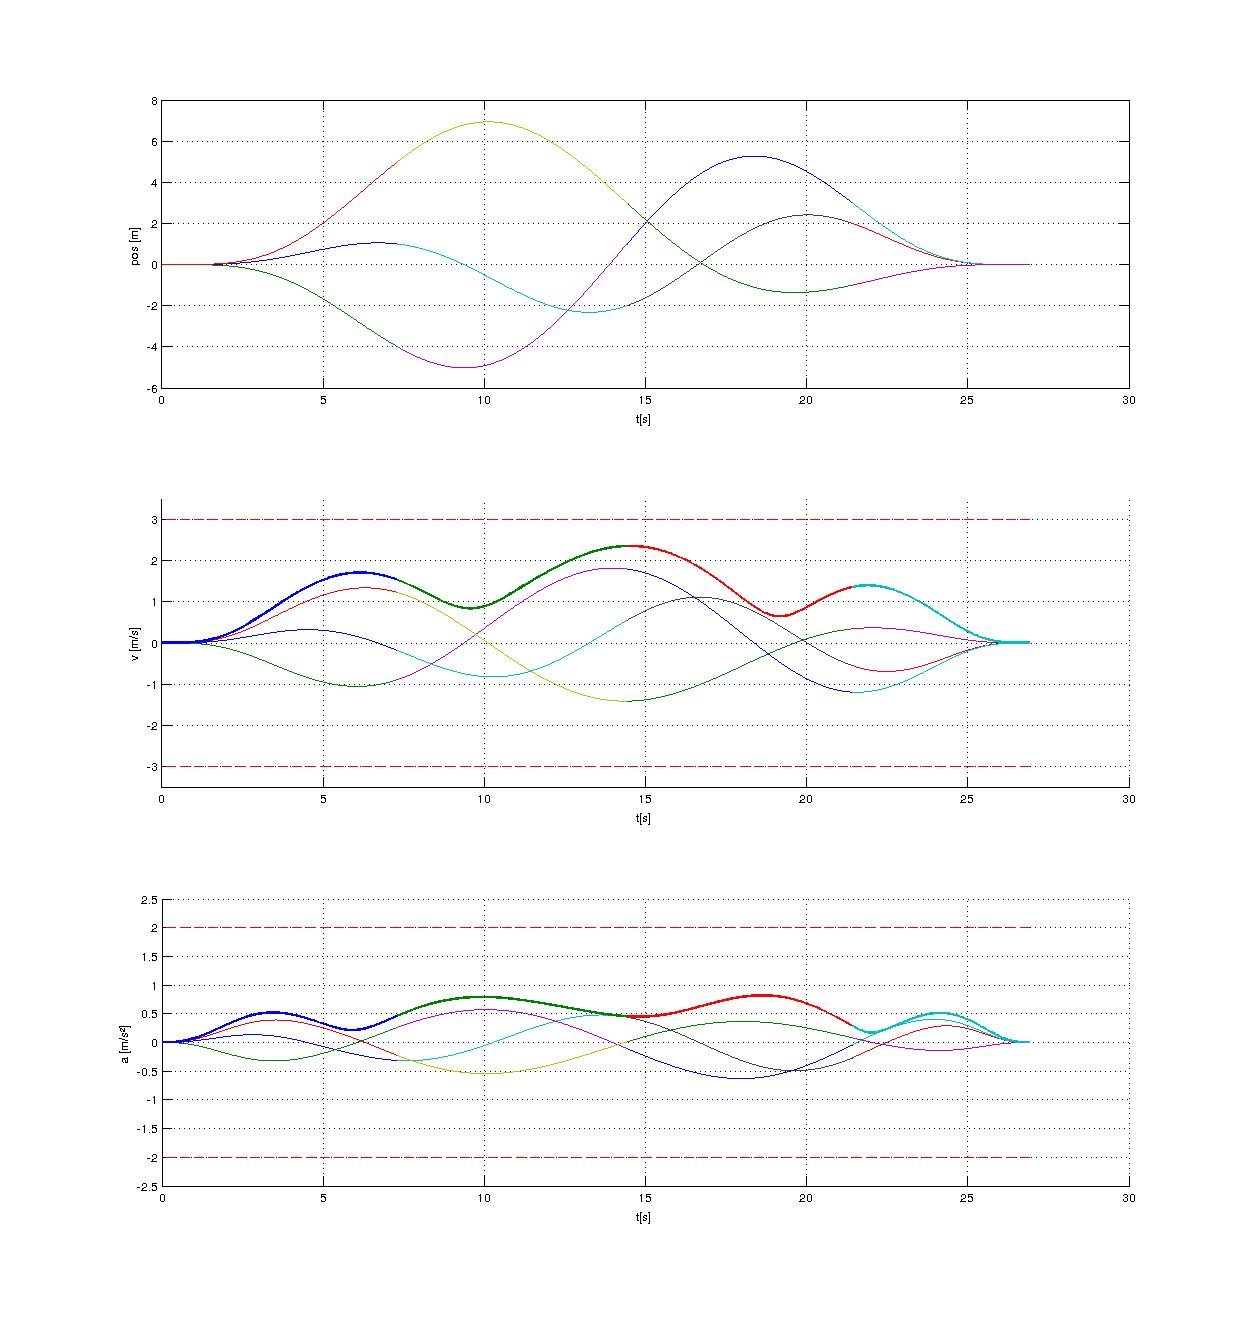
\includegraphics[scale=1]{pics/initial.eps}
%   \caption{Schematic of a rough foot surface.}
%   \label{pics:profile2}
%\end{figure}























